% ====================================================================
%  徐森林、薛春华《数学分析》（第一册）
%  \S2.5  有界闭区间 $[a,b]$ 上连续函数的性质
%  源：原书印刷页 135-150（PDF 物理页 141-156）
%  底本：高清影印比对校订
%  规范：全西文半角标点配合；单一落盘出口 _texout.py
% ====================================================================
\section{有界闭区间 $[a,b]$ 上连续函数的性质}\label{sec:2.5}

这一节主要研究有界闭区间 $[a,b]$ 上连续函数的重要定理: 零值定理、介值定理、最值定理、一致连续性定理以及它们的应用.

\begin{theorem}[零(根)值定理, Bolzano]\label{thm:2.5.1}
设 $f$ 为闭区间 $[a,b]$ 上的连续函数, 且 $f(a)f(b) < 0$, 则 $\exists \xi \in (a,b)$, 使得 $f(\xi) = 0$.
\end{theorem}

\begin{proof}
\textbf{证法 1}\quad 不妨设 $f(a) < 0, f(b) > 0$.

(反证) 假设 $f(x) \neq 0, \forall x \in (a,b)$. 现将 $[a,b]$ 两等分, 若 $f\left(\frac{a+b}{2}\right) > 0$, 则取 $a_1 = a$, $b_1 = \frac{a+b}{2}$; 若 $f\left(\frac{a+b}{2}\right) < 0$, 则取 $a_1 = \frac{a+b}{2}$, $b_1 = b$. 此时, $f(a_1) < 0$, $f(b_1) > 0$. 再将 $[a_1,b_1]$ 两等分, 若 $f\left(\frac{a_1+b_1}{2}\right) > 0$, 则取 $a_2 = a_1$, $b_2 = \frac{a_1+b_1}{2}$; 若 $f\left(\frac{a_1+b_1}{2}\right) < 0$, 则取 $a_2 = \frac{a_1+b_1}{2}$, $b_2 = b_1$, 此时, $f(a_2) < 0$, $f(b_2) > 0$. 如此下去, 得一递降闭区间套:
\[
[a,b] \supset [a_1,b_1] \supset [a_2,b_2] \supset \cdots \supset [a_n,b_n] \supset \cdots,
\]
$b_n - a_n = \frac{b-a}{2^n} \to 0\ (n \to +\infty)$, $f(a_n) < 0$, $f(b_n) > 0$. 根据实数连续性命题(三)(闭区间套原理)知, $\exists_1 x_0 \in \bigcap\limits_{n=1}^{\infty}[a_n,b_n] \subset [a,b]$, 显然,
\[
\lim_{n \to +\infty} a_n = x_0 = \lim_{n \to +\infty} b_n.
\]
由 $f$ 连续知, $0 \geqslant \lim\limits_{n \to +\infty} f(a_n) = f(x_0) = \lim\limits_{n \to +\infty} f(b_n) \geqslant 0$, 所以, 有 $f(x_0) = 0$. 又 $f(a) < 0, f(b) > 0$, 故 $x_0 \neq a, b$, 即 $x_0 \in (a,b)$, 这与假设相矛盾(如图~\ref{fig:2.5.1} 所示). 因此, 必有 $\xi \in (a,b)$, 使得 $f(\xi) = 0$.

\textbf{证法 2}\quad 不妨设 $f(a) < 0, f(b) > 0$, 根据实数连续性命题(一), 可令
\[
\xi = \sup\{x \in [a,b] \mid f(x) < 0\}.
\]
根据 $\sup$ 的定义, $\exists x_n \in [a,b], f(x_n) < 0, \{x_n\}$ 严格增趋于 $\xi$. 又由 $f$ 连续知, $\exists \delta > 0$, s.t.
\[
f|_{[a,a+\delta]} < 0,\quad f|_{(b-\delta,b)} > 0.
\]
所以, $\xi \in (a,b)$. 再由上确界的定义, 有 $f|_{(\xi,b)} > 0$. 最后, 由 $f$ 的连续性得到
\[
0 \geqslant \lim_{n \to +\infty} f(x_n) = f(\xi) = \lim_{x \to \xi^+} f(x) \geqslant 0,
\]
因此, $f(\xi) = 0$.

\textbf{证法 3}\quad (反证) 假设 $f(x) \neq 0, \forall x \in (a,b)$. $\forall x \in (a,b)$, 由 $f$ 连续知, $\exists \delta_x > 0$, s.t. $f$ 在 $(x - \delta_x, x + \delta_x) \cap [a,b]$ 上严格同号, 则开区间族
\[
\mathcal{I} = \{(x - \delta_x, x + \delta_x) \mid x \in [a,b]\}
\]
为 $[a,b]$ 上的一个开(区间)覆盖. 根据实数连续性命题(四)($[a,b]$ 的紧致性)知, 存在有限的子覆盖 $\mathcal{I}_1 = \{(x_i - \delta_{x_i}, x_i + \delta_{x_i}) \mid i = 1, 2, \cdots, k\}$. 不失一般性, 设 $a \in (x_1 - \delta_{x_1}, x_1 + \delta_{x_1})$. 如果 $[a,b] \subset (x_1 - \delta_{x_1}, x_1 + \delta_{x_1})$, 那么 $f|_{[a,b]}$ 与 $f(a)$ 严格同号, 从而 $f(a)f(b) > 0$, 这与题设 $f(a)f(b) < 0$ 相矛盾. 因此, $b \notin (x_1 - \delta_{x_1}, x_1 + \delta_{x_1})$, 从而 $x_1 + \delta_{x_1} \in (a,b)$. 不妨设 $x_1 + \delta_{x_1} \in (x_2 - \delta_{x_2}, x_2 + \delta_{x_2})$. 由于 $(x_1 - \delta_{x_1}, x_1 + \delta_{x_1}) \cap (x_2 - \delta_{x_2}, x_2 + \delta_{x_2}) \neq \varnothing$, 所以 $f$ 在 $(x_1 - \delta_{x_1}, x_1 + \delta_{x_1})$ 与 $(x_2 - \delta_{x_2}, x_2 + \delta_{x_2})$ 上严格同号. 依次得到一串开区间 $\{(x_i - \delta_{x_i}, x_i + \delta_{x_i}) \mid i = 1, \cdots, l\}$, 其中 $l \leqslant k$, $f$ 在这些开区间上依次是同号的, 并且 $b \in (x_l - \delta_{x_l}, x_l + \delta_{x_l})$, 所以 $f(a)$ 与 $f(b)$ 严格同号, 这与题设 $f(a)$ 与 $f(b)$ 严格异号相矛盾.
\end{proof}

\begin{figure}[htbp]
\centering
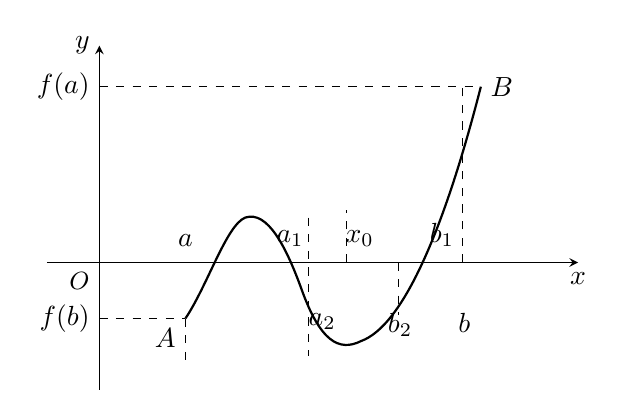
\begin{tikzpicture}[scale=0.95,>=stealth]
  \draw[->] (-0.7,0) -- (6.4,0) node[below] {$x$};
  \draw[->] (0,-1.7) -- (0,2.9) node[left] {$y$};
  \node[below left] at (0,0) {\small $O$};
  \draw[thick] (1.15,-0.75)
    .. controls (1.45,-0.30) and (1.70,0.50) .. (1.95,0.60)
    .. controls (2.25,0.70) and (2.50,0.20) .. (2.70,-0.35)
    .. controls (2.95,-1.05) and (3.20,-1.20) .. (3.50,-1.05)
    .. controls (4.05,-0.85) and (4.60,0.40) .. (5.10,2.35);
  \node[right] at (5.10,2.35) {$B$};
  \node[below left] at (1.15,-0.75) {$A$};
  \draw[dashed] (0,2.35) -- (5.10,2.35);
  \draw[dashed] (0,-0.75) -- (1.15,-0.75);
  \node[left] at (0,2.35) {$f(a)$};
  \node[left] at (0,-0.75) {$f(b)$};
  \draw[dashed] (1.15,-0.75) -- (1.15,-1.30);
  \node[above] at (1.15,0.08) {$a$};
  \draw[dashed] (2.80,0.60) -- (2.80,-1.25);
  \node[above] at (2.55,0.08) {$a_1$};
  \node[below] at (2.98,-0.55) {$a_2$};
  \draw[dashed] (3.30,0) -- (3.30,0.70);
  \node[above] at (3.48,0.08) {$x_0$};
  \draw[dashed] (4.00,0) -- (4.00,-0.70);
  \node[below] at (4.02,-0.55) {$b_2$};
  \draw[dashed] (4.85,0) -- (4.85,2.35);
  \node[above] at (4.58,0.08) {$b_1$};
  \node[below] at (4.88,-0.55) {$b$};
\end{tikzpicture}
\caption{}\label{fig:2.5.1}
\end{figure}

\begin{theoremp}[推广的零(根)值定理]\label{thm:2.5.1p}
设 $f$ 为 $[a,b]$ 上的连续函数, 且 $f(a)f(b) \leqslant 0$, 则 $\exists \xi \in [a,b]$, s.t. $f(\xi) = 0$.
\end{theoremp}

\begin{proof}
如果 $f(a) = 0$, 则取 $\xi = a$; 如果 $f(b) = 0$, 则取 $\xi = b$; 如果 $f(a)f(b) \neq 0$, 则 $f(a)f(b) < 0$, 由零值定理~\ref{thm:2.5.1} 知, $\exists \xi \in (a,b)$, s.t. $f(\xi) = 0$.
\end{proof}

\begin{theorem}[介值定理]\label{thm:2.5.2}
设 $f$ 为 $[a,b]$ 上的连续函数,\allowbreak $f(a) \neq f(b)$,\allowbreak 则 $\forall r \in (\min\{f(a), f(b)\},\allowbreak \max\{f(a), f(b)\})$, $\exists \xi \in (a,b)$, s.t. $f(\xi) = r$.
\end{theorem}

\begin{proof}
令 $F(x) = f(x) - r$, 显然它为 $[a,b]$ 上的连续函数, 且 $F(a)F(b) = (f(a) - r)(f(b) - r) < 0$. 由零值定理~\ref{thm:2.5.1} 知, $\exists \xi \in (a,b)$, s.t. $f(\xi) - r = F(\xi) = 0$, 即 $f(\xi) = r$(如图~\ref{fig:2.5.2} 所示).
\end{proof}

\begin{figure}[htbp]
\centering
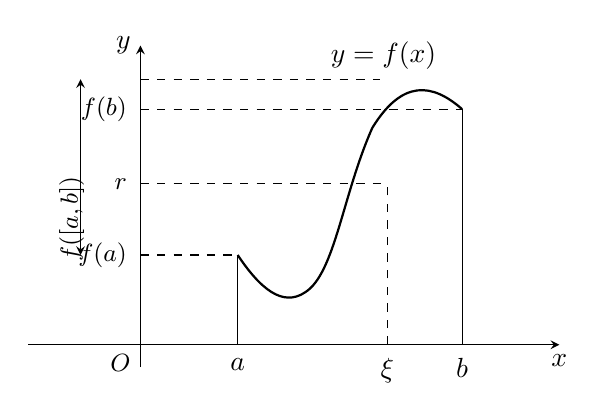
\begin{tikzpicture}[scale=0.95,>=stealth]
  \draw[->] (-1.5,0) -- (5.6,0) node[below] {$x$};
  \draw[->] (0,-0.3) -- (0,4.0) node[left] {$y$};
  \node[below left] at (0,0) {\small $O$};
  \draw[thick] (1.30,1.20)
    .. controls (1.60,0.75) and (1.90,0.50) .. (2.20,0.70)
    .. controls (2.60,0.95) and (2.70,2.00) .. (3.10,2.90)
    .. controls (3.50,3.55) and (3.90,3.50) .. (4.30,3.15);
  \node[above] at (3.25,3.55) {$y=f(x)$};
  \draw (1.30,1.20) -- (1.30,0);
  \draw (4.30,3.15) -- (4.30,0);
  \node[below] at (1.30,-0.05) {$a$};
  \node[below] at (4.30,-0.05) {$b$};
  \draw[dashed] (0,1.20) -- (1.32,1.20);
  \node[left,font=\small] at (-0.05,1.20) {$f(a)$};
  \draw[dashed] (0,3.15) -- (4.30,3.15);
  \node[left,font=\small] at (-0.05,3.15) {$f(b)$};
  \draw[dashed] (0,2.15) -- (3.30,2.15);
  \node[left,font=\small] at (-0.05,2.15) {$r$};
  \draw[dashed] (3.30,0) -- (3.30,2.15);
  \node[below] at (3.30,-0.05) {$\xi$};
  \draw[dashed] (0,3.55) -- (3.20,3.55);
  \draw[<->] (-0.80,1.20) -- (-0.80,3.55);
  \node[left,rotate=90,font=\small] at (-0.92,2.38) {$f([a,b])$};
\end{tikzpicture}
\caption{}\label{fig:2.5.2}
\end{figure}

\begin{theoremp}[推广的介值定理]\label{thm:2.5.2p}
设 $f$ 为 $[a,b]$ 上的连续函数,\allowbreak 则 $\forall r \in [\min\{f(a), f(b)\},\allowbreak \max\{f(a), f(b)\}]$, $\exists \xi \in [a,b]$, s.t. $f(\xi) = r$.
\end{theoremp}

\begin{proof}
不妨设 $f(a) \leqslant f(b)$. 如果 $r = \min\{f(a), f(b)\} = f(a)$, 则取 $\xi = a$; 如果 $r = \max\{f(a), f(b)\} = f(b)$, 则取 $\xi = b$. 如果 $f(a) = \min\{f(a), f(b)\} < r < \max\{f(a), f(b)\} = f(b)$, 则由介值定理~\ref{thm:2.5.2} 知, $\exists \xi \in (a,b)$, s.t. $f(\xi) = r$.

或者将推广的零值定理~\ref{thm:2.5.1p} 用于函数 $F(x) = f(x) - r$ 知, $\exists \xi \in [a,b]$, s.t. $0 = F(\xi) = f(\xi) - r$, 即 $f(\xi) = r$.
\end{proof}

\begin{corollary}\label{cor:2.5.1}
设 $f$ 为区间 $I$(开或半开半闭或闭)上的连续函数, 则 $f$ 的值域 $f(I) = \{f(x) \mid x \in I\}$ 也为一个区间(可退缩为一点).
\end{corollary}

\begin{proof}
若 $f$ 为常值函数, 即 $f(x) \equiv c$(常数), 则 $f(I) = \{c\}$ 退缩为一点.

若 $f$ 不为常值函数, 则必有 $y_1, y_2 \in f(I)$, s.t. $y_1 < y_2$. 由推广的介值定理~\ref{thm:2.5.2p} 知, $\forall r \in [y_1, y_2]$, 必 $\exists \xi \in I$, s.t. $r = f(\xi) \in f(I)$. 所以, $[y_1, y_2] \subset f(I)$. 由 $y_1, y_2$ 的任意性知, $f(I)$ 为一个区间.
\end{proof}

\begin{theorem}[最值定理]\label{thm:2.5.3}
设 $f$ 为有界闭区间 $[a,b]$ 上的连续函数, 则 $f$ 在 $[a,b]$ 上必达到最大值与最小值, 即必存在 $x_*, x^* \in [a,b]$, s.t.
\[
f(x_*) = \min_{x \in [a,b]} f(x) = m,
\]
\[
f(x^*) = \max_{x \in [a,b]} f(x) = M.
\]
\end{theorem}

\begin{proof}
记 $M = \sup\limits_{x \in [a,b]} f(x)$, 则 $M > -\infty$. 任取实数列 $\{\alpha_n\}$, s.t. $\alpha_n < M$ 且 $\{\alpha_n\}$ 严格增趋于 $M$. $\forall n \in \mathbb{N}$, $\alpha_n$ 不是 $f$ 在 $[a,b]$ 上的上界, 故 $\exists x_n \in [a,b]$, s.t. $\alpha_n < f(x_n) \leqslant M$. $\{x_n \mid n \in \mathbb{N}\} \subset [a,b]$ 为有界数列, 根据实数连续性命题(六)(序列紧性)知, 它有收敛子列 $x_{n_k}$. 令 $\lim\limits_{k \to +\infty} x_{n_k} = x^* \in [a,b]$, 由夹逼定理得到 $\lim\limits_{n \to +\infty} f(x_n) = \lim\limits_{n \to +\infty} \alpha_n = M$. 于是, 根据 $f$ 的连续性, 有
\[
M = \lim_{k \to +\infty} f(x_{n_k}) = f(x^*) \leqslant M,
\]
\[
f(x^*) = M,
\]
即 $f(x^*)$ 为 $f$ 在 $[a,b]$ 上的最大值.

同理可证, $\exists x_* \in [a,b]$, s.t. $f(x_*) = m = \inf\limits_{x \in [a,b]} f(x)$, 或用 $-f$ 代 $f$ 再应用上述所得结果.
\end{proof}

由此知, $f$ 在 $[a,b]$ 上为有界函数, 再由介值定理立即得到 $f$ 的值域
\[
f([a,b]) = \left[\min_{x \in [a,b]} f(x), \max_{x \in [a,b]} f(x)\right] = [m, M]
\]
为一个闭区间(包括退缩为一点, 此时 $f$ 为常值函数).

\begin{example}[不动点存在定理, Brouwer]\label{ex:2.5.1}
设 $f$ 在 $[a,b]$ 上连续, 满足 $a \leqslant f(x) \leqslant b, \forall x \in [a,b]$, 即 $f([a,b]) \subset [a,b]$, 则 $\exists \xi \in [a,b]$, s.t. $f(\xi) = \xi$, 称 $\xi$ 为 $f$ 的不动点.
\end{example}

\begin{proof}
令 $F(x) = f(x) - x$, 由 $f$ 连续知, $F$ 连续, 又因 $F(a)F(b) = (f(a) - a)(f(b) - b) \leqslant 0$, 根据推广零值定理~\ref{thm:2.5.1p} 知, $\exists \xi \in [a,b]$, s.t.
\[
f(\xi) - \xi = F(\xi) = 0,
\]
即 $f(\xi) = \xi$(如图~\ref{fig:2.5.3} 所示).
\end{proof}

\begin{figure}[htbp]
\centering
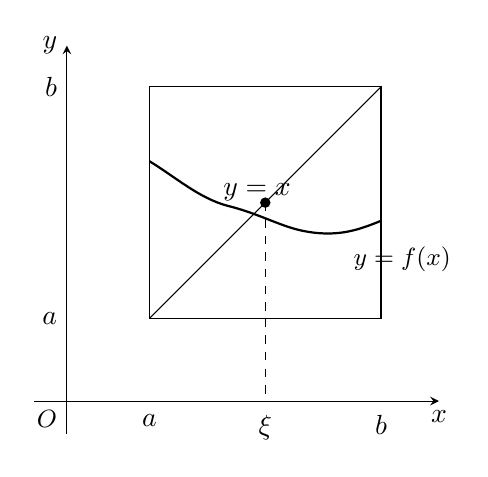
\begin{tikzpicture}[scale=1.05,>=stealth]
  \draw[->] (-0.4,0) -- (4.5,0) node[below] {$x$};
  \draw[->] (0,-0.4) -- (0,4.3) node[left] {$y$};
  \node[below left] at (0,0) {\small $O$};
  \draw (1.00,1.00) rectangle (3.80,3.80);
  \draw (1.00,1.00) -- (3.80,3.80);
  \node[above,sloped] at (2.30,2.30) {$y=x$};
  \draw[thick] (1.00,2.90)
    .. controls (1.30,2.72) and (1.60,2.45) .. (1.95,2.36)
    .. controls (2.35,2.26) and (2.60,2.10) .. (2.90,2.05)
    .. controls (3.30,1.98) and (3.55,2.08) .. (3.80,2.18);
  \node[below right,font=\small] at (3.35,1.98) {$y=f(x)$};
  \fill (2.40,2.40) circle (1.8pt);
  \draw[dashed] (2.40,2.40) -- (2.40,0);
  \node[below] at (1.00,-0.05) {$a$};
  \node[below] at (3.80,-0.05) {$b$};
  \node[below] at (2.40,-0.05) {$\xi$};
  \node[left] at (0,1.00) {$a$};
  \node[left] at (0,3.80) {$b$};
\end{tikzpicture}
\caption{}\label{fig:2.5.3}
\end{figure}

利用零值定理与介值定理可判断代数方程的根的存在范围.

\begin{example}\label{ex:2.5.2}
证明: 方程 $2^x = 4x$ 在 $\left(0, \frac{1}{2}\right)$ 中有根.
\end{example}

\begin{proof}
设 $f(x) = 2^x - 4x$, 它为初等函数, 因而是 $\left[0, \frac{1}{2}\right]$ 上的连续函数, 又 $f(0) = 2^0 - 4 \cdot 0 = 1 > 0$, $f\left(\frac{1}{2}\right) = 2^{\frac{1}{2}} - 4 \cdot \frac{1}{2} = \sqrt{2} - 2 < 0$, 则 $f(0)f\left(\frac{1}{2}\right) < 0$, 由零值定理~\ref{thm:2.5.1} 知, $\exists \xi \in \left(0, \frac{1}{2}\right)$, s.t.
\[
0 = f(\xi) = 2^{\xi} - 4\xi,
\]
即 $2^{\xi} = 4\xi, \xi \in \left(0, \frac{1}{2}\right)$ 为方程 $2^x = 4x$ 的一个根.
\end{proof}

\begin{example}\label{ex:2.5.3}
设 $f$ 在 $[a,b]$ 上连续, $x_1, x_2, \cdots, x_m \in [a,b]$, $\lambda_1, \lambda_2, \cdots, \lambda_m > 0$, $\sum\limits_{i=1}^{m} \lambda_i = 1$, 则 $\exists \xi \in [\min\{x_1, x_2, \cdots, x_m\}, \max\{x_1, x_2, \cdots, x_m\}] \subset [a,b]$, s.t.
\[
f(\xi) = \sum_{i=1}^{m} \lambda_i f(x_i).
\]
特别地, $\exists \xi \in [a,b]$, s.t. $f(\xi) = \frac{f(a) + f(b)}{2}$.
\end{example}

\begin{proof}
因为 $f$ 在 $[a,b]$ 上连续, 且
\[
\min\{f(x_1), f(x_2), \cdots, f(x_m)\} \leqslant \sum_{i=1}^{m} \lambda_i f(x_i) \leqslant \max\{f(x_1), f(x_2), \cdots, f(x_m)\},
\]
所以根据介值定理~\ref{thm:2.5.2} 知, $\exists \xi \in [\min\{x_1, x_2, \cdots, x_m\}, \max\{x_1, x_2, \cdots, x_m\}] \subset [a,b]$, s.t. $f(\xi) = \sum\limits_{i=1}^{m} \lambda_i f(x_i)$. 特别地, 当 $m = 2, x_1 = a, x_2 = b$, $\lambda_1 = \lambda_2 = \frac{1}{2}$ 时, $\exists \xi \in [a,b]$, s.t. $f(\xi) = \frac{f(a) + f(b)}{2}$.
\end{proof}

\begin{example}\label{ex:2.5.4}
证明: 实系数奇次多项式
\[
P(x) = x^{2n+1} + a_1 x^{2n} + \cdots + a_{2n} x + a_{2n+1}
\]
必有实根.
\end{example}

\begin{proof}
因为
\[
\lim_{x \to +\infty} P(x) = \lim_{x \to +\infty} x^{2n+1}\left(1 + \frac{a_1}{x} + \cdots + \frac{a_{2n}}{x^{2n}} + \frac{a_{2n+1}}{x^{2n+1}}\right) = +\infty,
\]
\[
\lim_{x \to -\infty} P(x) = \lim_{x \to -\infty} x^{2n+1}\left(1 + \frac{a_1}{x} + \cdots + \frac{a_{2n}}{x^{2n}} + \frac{a_{2n+1}}{x^{2n+1}}\right) = -\infty,
\]
故 $\exists \Delta > 0$, 当 $x > \Delta$ 时, $P(x) > 1$; 当 $x < -\Delta$ 时, $P(x) < -1$. 取 $a, b$, s.t. $a < -\Delta < \Delta < b$, 则 $P(a) < -1$, $P(b) > 1$. 又因多项式函数 $P(x)$ 为初等函数, 故它为 $\mathbb{R}$ 上的连续函数. 根据零值定理~\ref{thm:2.5.1}, $\exists \xi \in (a,b)$, s.t. $P(\xi) = 0$, 即实系数多项式 $P(x)$ 必有实根.
\end{proof}

\begin{example}\label{ex:2.5.5}
证明: $\tan x = x$ 有无穷个根.
\end{example}

\begin{proof}
设 $f(x) = \tan x - x, x \neq k\pi + \frac{\pi}{2}, k \in \mathbb{Z}$. 显然, 初等函数 $f(x) = \tan x - x$ 在其定义域中为连续函数, 因
\[
\lim_{x \to \left(k\pi + \frac{\pi}{2}\right)^-} (\tan x - x) = +\infty,
\]
\[
\lim_{x \to \left(k\pi - \frac{\pi}{2}\right)^+} (\tan x - x) = -\infty,
\]
故对每个固定的 $k \in \mathbb{Z}$, $\exists a_k, b_k$, s.t.
\[
k\pi - \frac{\pi}{2} < a_k < b_k < k\pi + \frac{\pi}{2},
\]
且 $f(a_k) < 0$, $f(b_k) > 0$. 根据零值定理~\ref{thm:2.5.1} 知, $\exists \xi_k \in (a_k, b_k) \subset \left(k\pi - \frac{\pi}{2}, k\pi + \frac{\pi}{2}\right)$, s.t.
\[
0 = f(\xi_k) = \tan \xi_k - \xi_k,
\]
即 $\tan \xi_k = \xi_k, k \in \mathbb{Z}$. 所以, $\tan x = x$ 有无穷个根(如图~\ref{fig:2.5.4} 所示).
\end{proof}

\begin{figure}[htbp]
\centering
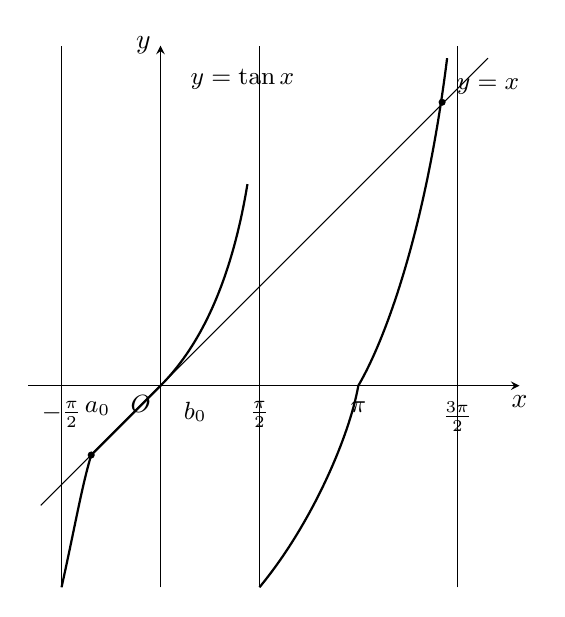
\begin{tikzpicture}[scale=0.80,>=stealth]
  \draw[->] (-2.1,0) -- (5.7,0) node[below] {$x$};
  \draw[->] (0,-3.2) -- (0,5.4) node[left] {$y$};
  \node[below left] at (0,0) {\small $O$};
  \draw (-1.571,-3.2) -- (-1.571,5.4);
  \draw (1.571,-3.2) -- (1.571,5.4);
  \draw (4.712,-3.2) -- (4.712,5.4);
  \draw[thick] (-1.571,-3.2)
     .. controls (-1.35,-2.20) and (-1.25,-1.60) .. (-1.10,-1.10)
     .. controls (-0.60,-0.60) and (-0.30,-0.30) .. (0,0)
     .. controls (0.55,0.55) and (1.10,1.50) .. (1.38,3.20);
  \draw[thick] (1.571,-3.2)
     .. controls (2.40,-2.20) and (3.00,-0.80) .. (3.14,0)
     .. controls (3.55,0.70) and (4.20,2.40) .. (4.55,5.20);
  \draw (-1.9,-1.9) -- (5.2,5.2);
  \node[right,font=\small] at (4.55,4.75) {$y=x$};
  \node[above,font=\small] at (1.30,4.55) {$y=\tan x$};
  \fill (-1.10,-1.10) circle (1.6pt);
  \fill (4.47,4.50) circle (1.6pt);
  \node[below,font=\small] at (-1.571,-0.10) {$-\frac{\pi}{2}$};
  \node[below,font=\small] at (-1.00,-0.10) {$a_0$};
  \node[below,font=\small] at (0.55,-0.10) {$b_0$};
  \node[below,font=\small] at (1.571,-0.10) {$\frac{\pi}{2}$};
  \node[below,font=\small] at (3.14,-0.10) {$\pi$};
  \node[below,font=\small] at (4.712,-0.10) {$\frac{3\pi}{2}$};
\end{tikzpicture}
\caption{}\label{fig:2.5.4}
\end{figure}

\begin{example}\label{ex:2.5.6}
设函数 $f$ 在 $(a,b)$ 上连续, 且 $f(a^+), f(b^-)$ 存在有限, 则 $f$ 在 $(a,b)$ 上有界.
\end{example}

\begin{proof}
\textbf{证法 1}\quad 令
\[
\tilde{f}(x) = \begin{cases} f(x), & x \in (a,b), \\ f(a^+), & x = a, \\ f(b^-), & x = b. \end{cases}
\]
显然, $\tilde{f}$ 在 $[a,b]$ 上连续, 根据最值定理~\ref{thm:2.5.3} 知, $\exists x_*, x^* \in [a,b]$, s.t. $\tilde{f}(x_*) = \min\limits_{x \in [a,b]} \tilde{f}(x) \leqslant f(x) \leqslant \max\limits_{x \in [a,b]} \tilde{f}(x) = \tilde{f}(x^*)$, $\forall x \in (a,b)$, 从而, $f$ 在 $(a,b)$ 上有界.

\textbf{证法 2}\quad 因 $f(a^+), f(b^-)$ 存在有限, 所以, 对 $\varepsilon_0 = 1$, $\exists \delta > 0$, s.t. $a < a + \delta < b - \delta < b$, 且
\[
f(a^+) - 1 < f(x) < f(a^+) + 1, \quad a < x < a + \delta,
\]
\[
f(b^-) - 1 < f(x) < f(b^-) + 1, \quad b - \delta < x < b.
\]
由 $f$ 在 $[a+\delta, b-\delta]$ 上连续, 并根据最值定理~\ref{thm:2.5.3} 知,
\[
|f(x)| \leqslant L, \forall x \in [a+\delta, b-\delta].
\]
所以, $|f(x)| \leqslant M = \max\{L, |f(a^+) - 1|, |f(a^+) + 1|, |f(b^-) - 1|, |f(b^-) + 1|\}$, 即 $f$ 在 $(a,b)$ 上有界.
\end{proof}

\begin{example}\label{ex:2.5.7}
设 $f$ 在 $(-\infty, +\infty)$ 上连续, 且 $\lim\limits_{x \to \infty} f(x)$ 存在有限, 则 $f$ 在 $(-\infty, +\infty)$ 上有界, 且 $f$ 在 $(-\infty, +\infty)$ 上必达到最大值或最小值.
\end{example}

\begin{proof}
设 $\lim\limits_{x \to \infty} f(x) = a \in \mathbb{R}$.

如果 $f(x) \equiv a, \forall x \in (-\infty, +\infty)$, 则 $f$ 在 $(-\infty, +\infty)$ 上有界, 且 $f$ 在其上达到最大值或最小值 $a$.

如果 $f(x) \not\equiv a$, 则 $\exists x_0 \in (-\infty, +\infty)$, s.t. $f(x_0) \neq a$.

若 $f(x_0) < a$, 取 $\varepsilon_0 \in (0, a - f(x_0))$, 因为 $\lim\limits_{x \to \infty} f(x) = a$, 故 $\exists \Delta > 0$, 当 $|x| > \Delta$ 时, 有 $f(x) > a - \varepsilon_0 > a - (a - f(x_0)) = f(x_0)$. 又因 $f$ 连续, 并根据最值定理~\ref{thm:2.5.3} 知, $\exists x_* \in [-\Delta, \Delta]$, s.t.
\[
f(x_*) = \min_{x \in [-\Delta, \Delta]} f(x) \leqslant f(x_0).
\]
于是(如图~\ref{fig:2.5.5} 所示),
\[
f(x_*) = \min_{x \in (-\infty, +\infty)} f(x).
\]
若 $f(x_0) > a$, 类似上述证明或用 $-f$ 代 $f$ 得 $x^* \in (-\infty, +\infty)$, s.t.
\[
f(x^*) = \max_{x \in (-\infty, +\infty)} f(x).
\]
\end{proof}

\begin{figure}[htbp]
\centering
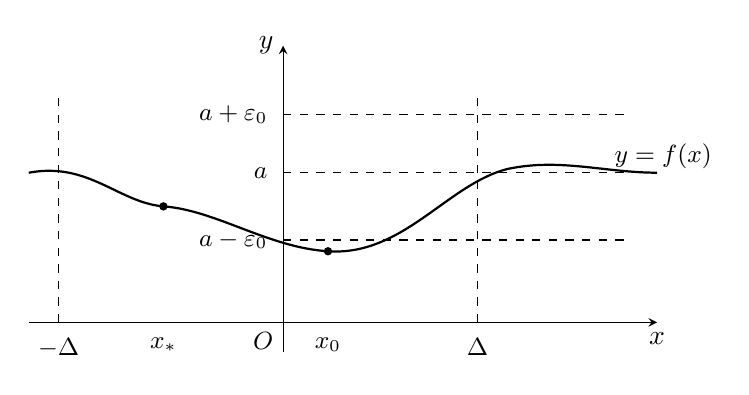
\begin{tikzpicture}[scale=0.95,>=stealth]
  \draw[->] (-3.4,0) -- (5.0,0) node[below] {$x$};
  \draw[->] (0,-0.4) -- (0,3.7) node[left] {$y$};
  \node[below left] at (0,0) {\small $O$};
  \draw[thick] (-3.4,2.00)
     .. controls (-2.60,2.15) and (-2.20,1.60) .. (-1.60,1.55)
     .. controls (-0.90,1.50) and (-0.20,1.00) .. (0.60,0.95)
     .. controls (1.60,0.88) and (2.20,1.85) .. (3.00,2.05)
     .. controls (3.70,2.20) and (4.30,2.00) .. (5.0,2.00);
  \node[right,font=\small] at (4.30,2.22) {$y=f(x)$};
  \draw[dashed] (0,2.00) -- (5.0,2.00);
  \draw[dashed] (0,2.78) -- (4.60,2.78);
  \draw[dashed] (0,1.10) -- (4.60,1.10);
  \node[left,font=\small] at (-0.08,2.00) {$a$};
  \node[left,font=\small] at (-0.08,2.78) {$a+\varepsilon_0$};
  \node[left,font=\small] at (-0.08,1.10) {$a-\varepsilon_0$};
  \draw[dashed] (-3.00,0) -- (-3.00,3.10);
  \draw[dashed] (2.60,0) -- (2.60,3.10);
  \node[below,font=\small] at (-3.00,-0.08) {$-\Delta$};
  \node[below,font=\small] at (2.60,-0.08) {$\Delta$};
  \fill (-1.60,1.55) circle (1.6pt);
  \node[below,font=\small] at (-1.60,-0.08) {$x_*$};
  \fill (0.60,0.95) circle (1.6pt);
  \node[below,font=\small] at (0.60,-0.08) {$x_0$};
\end{tikzpicture}
\caption{}\label{fig:2.5.5}
\end{figure}

为了讨论有界闭区间 $[a,b]$ 上另一个重要的一致连续性定理, 我们先引进一致连续的概念.

\begin{definition}\label{def:2.5.1}
设 $X \subsetneq \mathbb{R}$, $f\colon X \to \mathbb{R}$ 为一元函数. 如果 $\forall \varepsilon > 0$, $\exists \delta = \delta(\varepsilon) > 0$($\delta(\varepsilon)$ 只与 $\varepsilon$ 有关, 而与 $X$ 中的点 $x$ 无关!), 当 $x', x'' \in X$, 且 $x'$ 与 $x''$ 之间的距离 $\rho(x', x'') = |x' - x''|$ 小于 $\delta$, 就有 $|f(x') - f(x'')| < \varepsilon$, 则称 $f$ 在 $X$ 上是\textbf{一致连续}(或\textbf{均匀连续})的.
\end{definition}

\begin{theorem}\label{thm:2.5.4}
如果 $f$ 在 $X$ 上一致连续, 则 $f$ 在 $X$ 上连续. 但反之不真.
\end{theorem}

\begin{proof}
$\forall \varepsilon > 0$, 因 $f$ 在 $X$ 上一致连续, 故 $\exists \delta = \delta(\varepsilon) > 0$, 当 $x', x'' \in X, |x' - x''| < \delta$ 时, 有 $|f(x') - f(x'')| < \varepsilon$. 对 $x_0 \in X$, 当 $x \in X, |x - x_0| < \delta$ 时, 当然有 $|f(x) - f(x_0)| < \varepsilon$, 这就证明了 $f$ 在 $\forall x_0 \in X$ 处是连续的, 即 $f$ 在 $X$ 上连续.
\end{proof}

反之不真有反例: $f(x) = \frac{1}{x}$. 显然, 基本初等函数 $\frac{1}{x} = x^{-1}$ 在 $(0,1)$ 上连续. 但是, 它在 $(0,1)$ 上不一致连续.

\textbf{证法 1}\quad (反证) 假设 $f(x) = \frac{1}{x}$ 在 $(0,1)$ 上一致连续, 对 $\forall \varepsilon > 0, \exists \delta = \delta(\varepsilon) > 0$, 当 $x', x'' \in (0,1), |x' - x''| < \delta$ 时, 有
\[
\left|\frac{1}{x'} - \frac{1}{x''}\right| = |f(x') - f(x'')| < \varepsilon.
\]
取定 $x'' \in (0, \delta)$, 令 $x' \to 0^+$, 得到 $+\infty \leqslant \varepsilon$, 矛盾.

\textbf{证法 2}\quad 取 $\varepsilon_0 = 1, \forall \delta \in \left(0, \frac{1}{2}\right)$, 当 $x' = \frac{\delta}{2}, x'' = \delta$ 时, 虽然 $|x' - x''| = \left|\frac{\delta}{2} - \delta\right| = \frac{\delta}{2} < \delta$, 但
\[
\left|\frac{1}{x'} - \frac{1}{x''}\right| = \left|\frac{1}{\frac{\delta}{2}} - \frac{1}{\delta}\right| = \frac{1}{\delta} > 2 > 1 = \varepsilon_0.
\]
所以, $f(x) = \frac{1}{x}$ 在 $(0,1)$ 上不一致连续.

\textbf{证法 3}\quad 取 $x_n' = \frac{1}{n}, x_n'' = \frac{1}{n+1}$, 虽然
\[
|x_n' - x_n''| = \left|\frac{1}{n} - \frac{1}{n+1}\right| = \frac{1}{n(n+1)} \to 0 \quad (n \to +\infty),
\]
但
\[
|f(x_n') - f(x_n'')| = \left|\frac{1}{\frac{1}{n}} - \frac{1}{\frac{1}{n+1}}\right| = |n - (n+1)| = 1 \not\to 0 \quad (n \to +\infty).
\]
根据下面的定理~\ref{thm:2.5.8} 知, $f(x) = \frac{1}{x}$ 在 $(0,1)$ 上不一致连续.

\begin{theorem}[Cantor 定理]\label{thm:2.5.5}
有界闭区间 $[a,b]$ 上的连续函数是一致连续的.
\end{theorem}

\begin{proof}
\textbf{证法 1}\quad (反证) 假设 $f$ 在 $[a,b]$ 上不一致连续, 根据其定义知, $\exists \varepsilon_0 > 0, \forall n \in \mathbb{N}$, $\exists x_n', x_n'' \in [a,b]$, 虽然 $|x_n' - x_n''| < \frac{1}{n}$, 但
\[
|f(x_n') - f(x_n'')| \geqslant \varepsilon_0.
\]
由于数列 $\{x_n'\}$ 有界, 根据实数连续性命题(六)(序列紧性)知, 存在收敛子列 $\{x_{n_k}'\}$, 记
\[
\lim_{k \to +\infty} x_{n_k}' = x_0 \in [a,b].
\]
另一方面, 由于 $|x_{n_k}' - x_{n_k}''| < \frac{1}{n_k} \leqslant \frac{1}{k} \to 0\ (k \to +\infty)$, 故有 $\lim\limits_{k \to +\infty} x_{n_k}'' = x_0$, 但由上式知, $|f(x_{n_k}') - f(x_{n_k}'')| \geqslant \varepsilon_0$. 所以, 由 $f$ 连续得到
\[
0 = |f(x_0) - f(x_0)| = \lim_{k \to +\infty} |f(x_{n_k}') - f(x_{n_k}'')| \geqslant \varepsilon_0 > 0,
\]
矛盾.

\textbf{证法 2}\quad 因 $f$ 在 $[a,b]$ 上连续, 故 $\forall \varepsilon > 0, \forall x \in [a,b], \exists \delta_x > 0$, s.t. 当 $u \in [a,b] \cap (x - \delta_x, x + \delta_x)$ 时, $|f(u) - f(x)| < \frac{\varepsilon}{2}$. 当 $x', x'' \in [a,b] \cap (x - \delta_x, x + \delta_x)$ 时,
\[
\begin{aligned}
|f(x') - f(x'')| &\leqslant |f(x') - f(x)| + |f(x'') - f(x)| \\
&< \frac{\varepsilon}{2} + \frac{\varepsilon}{2} = \varepsilon.
\end{aligned}
\tag*{(*)}
\]
显然, $\mathcal{I} = \left\{\left(x - \frac{\delta_x}{2}, x + \frac{\delta_x}{2}\right) \mid x \in [a,b]\right\}$ 为 $[a,b]$ 的一个开区间覆盖. 由实数连续性命题(四)($[a,b]$ 的紧致性)知, 存在有限子覆盖 $\mathcal{I}_1 = \left\{\left(x_k - \frac{\delta_{x_k}}{2}, x_k + \frac{\delta_{x_k}}{2}\right) \mid k = 1, 2, \cdots, n\right\} \subset \mathcal{I}$. 令
\[
\delta = \delta(\varepsilon) = \min\left\{\frac{\delta_{x_k}}{2} \mid k = 1, 2, \cdots, n\right\} > 0,
\]
则 $\forall x', x'' \in [a,b], |x' - x''| < \delta$, $\exists k \in \mathbb{N}, 1 \leqslant k \leqslant n$, s.t.
\[
x' \in \left(x_k - \frac{\delta_{x_k}}{2}, x_k + \frac{\delta_{x_k}}{2}\right).
\]
于是,
\[
|x'' - x_k| \leqslant |x'' - x'| + |x' - x_k| < \delta + \frac{\delta_{x_k}}{2} \leqslant \delta_{x_k},
\]
即 $x'' \in (x_k - \delta_{x_k}, x_k + \delta_{x_k})$, 由 $(*)$ 式推得
\[
|f(x') - f(x'')| < \varepsilon,
\]
从而 $f$ 在 $[a,b]$ 上一致连续.

\textbf{证法 3}\quad 在证法 2 中, 令
\[
\tilde{\mathcal{I}} = \{(x - \delta_x, x + \delta_x) \mid x \in [a,b]\},
\]
则 $\tilde{\mathcal{I}}$ 为 $[a,b]$ 的开区间覆盖. 根据下面的 Lebesgue 数定理~\ref{thm:2.5.6} 知, 存在 Lebesgue 数 $\lambda = \lambda(\mathcal{I}) > 0$. $\forall \varepsilon > 0$, 取 $\delta = \delta(\varepsilon) = \lambda(\tilde{\mathcal{I}})$, 则当 $x', x'' \in [a,b]$ 且两点集 $\{x', x''\}$ 的直径为
\[
d(\{x', x''\}) = |x' - x''| < \delta = \lambda(\tilde{\mathcal{I}})
\]
时, 必有 $(x_0 - \delta_{x_0}, x_0 + \delta_{x_0}) \in \tilde{\mathcal{I}}$, s.t. $\{x', x''\} \subset (x_0 - \delta_{x_0}, x_0 + \delta_{x_0})$, 从而,
\[
|f(x') - f(x'')| < \varepsilon.
\]
这就证明了 $f$ 在 $[a,b]$ 上是一致连续的.
\end{proof}

\begin{theorem}[Lebesgue 数定理]\label{thm:2.5.6}
设 $\mathcal{I}$ 为有界闭区间 $[a,b]$ 上的一个开覆盖, 则必存在数 $\lambda = \lambda(\mathcal{I}) > 0$, 使当集合 $A \subset [a,b]$, 其直径 $d(A) = \sup\{\rho(x', x'') \mid x', x'' \in A\} < \lambda = \lambda(\mathcal{I})$ 时, 必有 $I \in \mathcal{I}$, s.t. $A \subset I$. 我们称 $\lambda = \lambda(\mathcal{I})$ 为 $\mathcal{I}$ 的一个 Lebesgue 数.
\end{theorem}

\begin{proof}
(反证) 假设结论不成立, 则 $\forall n \in \mathbb{N}$, 存在 $A_n \subset [a,b]$, 它的直径 $d(A_n) < \frac{1}{n}$, 而不存在 $I \in \mathcal{I}$, s.t. $A_n \subset I$. 在每个 $A_n$ 中取 $a_n$, 根据实数连续性命题(六)(序列紧性)可知, 存在子列 $\{a_{n_k}\}$ 收敛于 $a_0 \in [a,b]$. 因为 $\mathcal{I}$ 为 $[a,b]$ 的开覆盖, 故存在 $I_0 \in \mathcal{I}$, 使得 $a_0 \in I_0$. 因为 $I_0$ 为开集, 当 $[a,b] \setminus I_0 \neq \varnothing$ 时, 点 $a_0$ 到 $[a,b] \setminus I_0$ 的距离
\[
d = \rho(a_0, [a,b] \setminus I_0) = \inf\{\rho(a_0, x) \mid x \in [a,b] \setminus I_0\} > 0.
\]
由于 $\lim\limits_{k \to +\infty} a_{n_k} = a_0$, 所以, $\exists n_{k_0}$, s.t. $n_{k_0} > \frac{2}{d}$ 与 $\rho(a_0, a_{n_{k_0}}) < \frac{d}{2}$. 于是, $\forall x \in A_{n_{k_0}}$, 有
\[
\rho(a_0, x) \leqslant \rho(a_0, a_{n_{k_0}}) + \rho(a_{n_{k_0}}, x) < \frac{d}{2} + \frac{1}{n_{k_0}} < \frac{d}{2} + \frac{d}{2} = d,
\]
因而, $A_{n_{k_0}} \subset I_0 \in \mathcal{I}$; 当 $[a,b] \setminus I_0 = \varnothing$ 时, $A_n \subset [a,b] \subset I_0$, 这与不存在 $I \in \mathcal{I}$ 使得 $A_{n_{k_0}} \subset I$ 相矛盾.
\end{proof}

\begin{theorem}\label{thm:2.5.7}
$f$ 在 $(a,b)$ 上一致连续 $\iff f$ 可延拓为 $[a,b]$ 上的连续函数 $\tilde{f}$, 此时 $\tilde{f}|_{(a,b)} = f|_{(a,b)}$.
\end{theorem}

\begin{proof}
($\Leftarrow$) 设 $f$ 可延拓为 $[a,b]$ 上的连续函数 $\tilde{f}$, 由 Cantor 定理~\ref{thm:2.5.5} 知, $\tilde{f}$ 在 $[a,b]$ 上一致连续, 而 $\tilde{f}|_{(a,b)} = f|_{(a,b)}$, 因此 $f$ 在 $(a,b)$ 上一致连续.

($\Rightarrow$) 设 $f$ 在 $(a,b)$ 上一致连续. $\forall \varepsilon > 0$, $\exists \delta = \delta(\varepsilon) > 0$, 当 $x', x'' \in (a,b), |x' - x''| < \delta$ 时, $|f(x') - f(x'')| < \varepsilon$.

任取 $x_n \in (a,b)$, $x_n \to a^+$, 则 $\{x_n\}$ 为 Cauchy(基本)数列. 因此, $\exists N \in \mathbb{N}$, 当 $m, n > N$ 时, $|x_n - x_m| < \delta$, 从而有 $|f(x_n) - f(x_m)| < \varepsilon$. 这就证明了 $\{f(x_n)\}$ 为 Cauchy(基本)数列. 根据实数连续性命题(七)($\mathbb{R}$ 的完备性)知, $\{f(x_n)\}$ 收敛. $\forall x_n', x_n'' \to a^+\ (n \to +\infty)$, 显然有
\[
\{x_n'''\} \colon x_1', x_1'', x_2', x_2'', \cdots, x_n', x_n'', \cdots \to a^+.
\]
由上证得 $\{f(x_n''')\}$ 收敛, 并且
\[
\lim_{n \to +\infty} f(x_n') = \lim_{n \to +\infty} f(x_n'') = \lim_{n \to +\infty} f(x_n''').
\]
这就证明了 $\forall x_n \to a^+$, $\{f(x_n)\}$ 收敛于同一数, 故 $\lim\limits_{x \to a^+} f(x)$ 存在有限. 同理可证 $\lim\limits_{x \to b^-} f(x)$ 存在有限. 令
\[
\tilde{f}(x) = \begin{cases} f(a^+), & x = a, \\ f(x), & a < x < b, \\ f(b^-), & x = b. \end{cases}
\]
显然, $\tilde{f}$ 为 $[a,b]$ 上的连续函数, 且为 $f$ 的延拓.
\end{proof}

\begin{theorem}\label{thm:2.5.8}
设 $X \subsetneq \mathbb{R}$, $f\colon X \to \mathbb{R}$ 为一元函数. 如果 $\exists x_n', x_n'' \in X, n \in \mathbb{N}$, $|x_n' - x_n''| \to 0$ 但 $|f(x_n') - f(x_n'')| \not\to 0\ (n \to +\infty)$, 则 $f$ 在 $X$ 上不一致连续.
\end{theorem}

\begin{proof}
(反证) 假设 $f$ 在 $X$ 上一致连续, 则 $\forall \varepsilon > 0, \exists \delta = \delta(\varepsilon) > 0$, 当 $x', x'' \in X, |x' - x''| < \delta$ 时, $|f(x') - f(x'')| < \varepsilon$. 因 $|x_n' - x_n''| \to 0\ (n \to +\infty)$, 故 $\exists N \in \mathbb{N}$, 当 $n > N$ 时, $|x_n' - x_n''| < \delta$, 从而有
\[
|f(x_n') - f(x_n'')| < \varepsilon.
\]
由此就推得 $|f(x_n') - f(x_n'')| \to 0\ (n \to +\infty)$, 这与题设 $|f(x_n') - f(x_n'')| \not\to 0\ (n \to +\infty)$ 相矛盾.
\end{proof}

\begin{example}\label{ex:2.5.8}
设 $X \subsetneq \mathbb{R}$, $f\colon X \to \mathbb{R}$ 为一元函数, 它满足 Lipschitz 条件, 即 $\forall x', x'' \in X$, 有 $|f(x') - f(x'')| \leqslant M|x' - x''|$, 其中 $M$ 为常数, 则 $f$ 在 $X$ 上为一致连续函数.
\end{example}

\begin{proof}
$\forall \varepsilon > 0$, 取 $\delta \in \left(0, \frac{\varepsilon}{M+1}\right)$, 当 $x', x'' \in X$, 且 $|x' - x''| < \delta$ 时,
\[
|f(x') - f(x'')| \leqslant M|x' - x''| \leqslant M\delta < M \cdot \frac{\varepsilon}{M+1} < \varepsilon.
\]
因此, $f$ 在 $X$ 上为一致连续函数.
\end{proof}

\begin{example}\label{ex:2.5.9}
(1) $f(x) = \frac{1}{x}$ 在 $[a,b]$ 上一致连续, $0 < a < b$;

(2) $f(x) = ax + b$ 在 $(-\infty, +\infty)$ 内一致连续;

(3) $f(x) = x^2$ 在 $(-\infty, +\infty)$ 内不一致连续;

(4) $f(x) = \sin x^2$ 在 $(-\infty, +\infty)$ 内不一致连续;

(5) $f(x) = \sin \frac{1}{x}$ 在 $(0,1)$ 上不一致连续.
\end{example}

\begin{proof}
(1) $\forall \varepsilon > 0$, 取 $\delta \in (0, a^2\varepsilon)$, 当 $x', x'' \in [a,b], |x' - x''| < \delta$ 时,
\[
\left|\frac{1}{x'} - \frac{1}{x''}\right| = \frac{|x' - x''|}{x'x''} \leqslant \frac{|x' - x''|}{a^2} < \frac{\delta}{a^2} < \varepsilon,
\]
所以, $f(x) = \frac{1}{x}$ 在 $[a,b]$ 上一致连续.

(2) $\forall \varepsilon > 0$, 取 $\delta \in \left(0, \frac{\varepsilon}{|a|+1}\right)$, 当 $x', x'' \in (-\infty, +\infty), |x' - x''| < \delta$ 时,
\[
\begin{aligned}
|f(x') - f(x'')| &= |(ax' + b) - (ax'' + b)| = |ax' - ax''| \\
&= |a| \cdot |x' - x''| \leqslant (|a| + 1)\delta < \varepsilon,
\end{aligned}
\]
所以, $f(x) = ax + b$ 在 $(-\infty, +\infty)$ 内一致连续.

(3) 取 $x_n' = n, x_n'' = n + \frac{1}{n}$, 则 $|x_n' - x_n''| = \left|n - \left(n + \frac{1}{n}\right)\right| = \frac{1}{n} \to 0\ (n \to +\infty)$, 而
\[
|f(x_n') - f(x_n'')| = \left|n^2 - \left(n + \frac{1}{n}\right)^2\right| = 2 + \frac{1}{n^2} \to 2 \neq 0 \quad (n \to +\infty).
\]
根据定理~\ref{thm:2.5.8} 知, $f(x) = x^2$ 在 $(-\infty, +\infty)$ 内不一致连续.

(4) 取 $x_n' = \sqrt{2n\pi + \frac{\pi}{2}}, x_n'' = \sqrt{2n\pi}$, 则
\[
\begin{aligned}
|x_n' - x_n''| &= \left|\sqrt{2n\pi + \frac{\pi}{2}} - \sqrt{2n\pi}\right| \\
&= \frac{\frac{\pi}{2}}{\sqrt{2n\pi + \frac{\pi}{2}} + \sqrt{2n\pi}} \to 0 \quad (n \to +\infty),
\end{aligned}
\]
但
\[
\begin{aligned}
|f(x_n') - f(x_n'')| &= |\sin(x_n')^2 - \sin(x_n'')^2| \\
&= \left|\sin\left(2n\pi + \frac{\pi}{2}\right) - \sin 2n\pi\right| \\
&= |1 - 0| = 1 \not\to 0 \quad (n \to +\infty),
\end{aligned}
\]
根据定理~\ref{thm:2.5.8} 知, $f(x) = \sin x^2$ 在 $(-\infty, +\infty)$ 内不一致连续.

(5) \textbf{证法 1}\quad 取 $x_n' = \frac{1}{2n\pi}, x_n'' = \frac{1}{2n\pi + \frac{\pi}{2}}$, 则
\[
|x_n' - x_n''| = \left|\frac{1}{2n\pi} - \frac{1}{2n\pi + \frac{\pi}{2}}\right| = \frac{\frac{\pi}{2}}{2n\pi\left(2n\pi + \frac{\pi}{2}\right)} \to 0 \quad (n \to +\infty),
\]
但
\[
\begin{aligned}
|f(x_n') - f(x_n'')| &= \left|\sin\frac{1}{x_n'} - \sin\frac{1}{x_n''}\right| = \left|\sin 2n\pi - \sin\left(2n\pi + \frac{\pi}{2}\right)\right| \\
&= |0 - 1| = 1 \not\to 0 \quad (n \to +\infty),
\end{aligned}
\]
根据定理~\ref{thm:2.5.8} 知, $f(x) = \sin\frac{1}{x}$ 在 $(0,1)$ 上不一致连续.

\textbf{证法 2}\quad (反证) 假设 $f(x) = \sin\frac{1}{x}$ 在 $(0,1)$ 上一致连续, 由定理~\ref{thm:2.5.7} 知, $f(x)$ 可延拓为 $[0,1]$ 上的连续函数 $\tilde{f}(x)$, 因而 $\tilde{f}(0) = \lim\limits_{x \to 0^+} \tilde{f}(x) = \lim\limits_{x \to 0^+} \sin\frac{1}{x}$ 存在有限, 这与 $\lim\limits_{x \to 0^+} \sin\frac{1}{x}$ 显然不存在相矛盾.
\end{proof}

\begin{example}\label{ex:2.5.10}
设 $f$ 在 $[a,+\infty)$ 上连续, 且 $\lim\limits_{x \to +\infty} f(x)$ 存在有限, 则 $f$ 在 $[a,+\infty)$ 上一致连续.
\end{example}

\begin{proof}
\textbf{证法 1}\quad 因 $\lim\limits_{x \to +\infty} f(x) = A \in \mathbb{R}$, 故 $\forall \varepsilon > 0$, 必 $\exists \Delta > 0$, 当 $x > \Delta$ 时, 有 $|f(x) - A| < \frac{\varepsilon}{2}$.

又因 $f$ 连续, 根据 Cantor 定理~\ref{thm:2.5.5} 知, $f$ 在 $[a,\Delta]$ 上一致连续, 故 $\exists \delta_1 > 0$, 当 $x', x'' \in [a,\Delta], |x' - x''| < \delta_1$ 时, 有
\[
|f(x') - f(x'')| < \varepsilon.
\]
由于 $f$ 在点 $\Delta$ 处连续, 所以 $\exists \delta_2 > 0$, 当 $|x - \Delta| < \delta_2$ 时, 有
\[
|f(x) - f(\Delta)| < \frac{\varepsilon}{2}.
\]
令 $\delta = \min\{\delta_1, \delta_2\} > 0$, 当 $x', x'' \in [a,+\infty), |x' - x''| < \delta$ 时, 必有下面结论:

(1) $x', x'' \in (\Delta, +\infty)$, 则
\[
|f(x') - f(x'')| \leqslant |f(x') - A| + |f(x'') - A| < \frac{\varepsilon}{2} + \frac{\varepsilon}{2} = \varepsilon.
\]

(2) $x', x'' \in [a,\Delta]$, 则 $|f(x') - f(x'')| < \varepsilon$.

(3) $x' \in [a,\Delta], x'' \in [\Delta,+\infty)$, 则
\[
|x' - \Delta| < x'' - x' < \delta \leqslant \delta_2,
\]
\[
|f(x') - f(\Delta)| < \frac{\varepsilon}{2}.
\]
同理, $|f(x'') - f(\Delta)| < \frac{\varepsilon}{2}$. 因此,
\[
|f(x') - f(x'')| \leqslant |f(x') - f(\Delta)| + |f(x'') - f(\Delta)| < \frac{\varepsilon}{2} + \frac{\varepsilon}{2} = \varepsilon.
\]
这就证明了 $f$ 在 $[a,+\infty)$ 上是一致连续的.

\textbf{证法 2}\quad 因 $\lim\limits_{x \to +\infty} f(x) = A \in \mathbb{R}$, 故 $\forall \varepsilon > 0$, 必 $\exists \Delta > 0$, 当 $x > \Delta$ 时, 有 $|f(x) - A| < \frac{\varepsilon}{2}$.

又因 $f$ 连续, 根据 Cantor 定理~\ref{thm:2.5.5} 知, $f$ 在 $[a,\Delta+1]$ 上一致连续, 故 $\exists \delta_1 > 0$, 当 $x', x'' \in [a,\Delta+1], |x' - x''| < \delta_1$ 时, 有
\[
|f(x') - f(x'')| < \varepsilon.
\]
令 $\delta = \min\{1, \delta_1\}$, 当 $x', x'' \in [a,+\infty), x' < x'', |x' - x''| < \delta$ 时, 必有下面结论:

(1) $x', x'' \in (\Delta, +\infty)$, 则
\[
|f(x') - f(x'')| \leqslant |f(x') - A| + |f(x'') - A| < \frac{\varepsilon}{2} + \frac{\varepsilon}{2} = \varepsilon.
\]

(2) $x', x'' \in [a, \Delta+1]$, 则
\[
|f(x') - f(x'')| < \varepsilon.
\]

(3) 若 $a \leqslant x' < \Delta < \Delta + 1 < x''$, 则
\[
1 = (\Delta + 1) - \Delta < |x' - x''| < \delta \leqslant 1,
\]
矛盾. 由此推得这种情形不出现.

综合上述知, $f$ 在 $[a,+\infty)$ 上一致连续.
\end{proof}

\begin{example}\label{ex:2.5.11}
设 $f\colon (-\infty, +\infty) \to \mathbb{R}$ 是以 $T > 0$ 为周期的连续函数, 则 $f$ 在 $(-\infty, +\infty)$ 上一致连续.
\end{example}

\begin{proof}
\textbf{证法 1}\quad 因 $f$ 是以 $T > 0$ 为周期的函数, 根据 Cantor 定理~\ref{thm:2.5.5} 知, $\forall \varepsilon > 0, \exists \delta_1 > 0$, 当 $x', x'' \in [kT, (k+1)T], k \in \mathbb{Z}$ 时,
\[
|f(x') - f(x'')| < \varepsilon.
\]
$\forall kT, \exists \delta_2 > 0$, 当 $|x - kT| < \delta_2$ 时, 有
\[
|f(x) - f(kT)| < \frac{\varepsilon}{2}.
\]
于是, $\forall x', x'' \in (kT - \delta_2, kT + \delta_2)$,
\[
|f(x') - f(x'')| \leqslant |f(x') - f(kT)| + |f(x'') - f(kT)| < \frac{\varepsilon}{2} + \frac{\varepsilon}{2} = \varepsilon.
\]
令 $\delta = \min\{T, \delta_1, \delta_2\}$, 则当 $x', x'' \in (-\infty, +\infty)$, $x' \leqslant x''$, $|x' - x''| < \delta$ 时, 有下面结论:

(1) $x', x'' \in [kT, (k+1)T]$, 则 $|f(x') - f(x'')| < \varepsilon$;

(2) $x' \in [(k-1)T, kT], x'' \in [kT, (k+1)T]$, 则
\[
|x' - kT| \leqslant |x' - x''| < \delta \leqslant \delta_2,
\]
\[
|x'' - kT| \leqslant |x' - x''| < \delta \leqslant \delta_2,
\]
\[
|f(x') - f(x'')| < \varepsilon.
\]
这就证明了 $f$ 在 $(-\infty, +\infty)$ 上是一致连续的.

\textbf{证法 2}\quad 因 $f$ 在 $[0,2T]$ 内连续, 根据 Cantor 定理~\ref{thm:2.5.5} 知, $f$ 在 $[0,2T]$ 内一致连续, 故 $\forall \varepsilon > 0$, 取 $\delta_1 > 0$, 当 $x', x'' \in [0,2T], |x' - x''| < \delta_1$ 时, 有 $|f(x') - f(x'')| < \varepsilon$.

令 $\delta = \min\{T, \delta_1\}$, 当 $x', x'' \in (-\infty, +\infty)$, $x' < x''$, 且 $|x' - x''| < \delta$ 时, 必有 $n \in \mathbb{Z}$, s.t. $x' = nT + x_0'$, 其中 $x_0' \in [0, T]$, 则 $x'' = nT + x_0''$, $x_0'' \in [0, 2T]$. 于是, $|x_0' - x_0''| = |(x' - nT) - (x'' - nT)| = |x' - x''| < \delta$,
\[
|f(x') - f(x'')| = |f(x_0') - f(x_0'')| < \varepsilon.
\]
这就证明了 $f$ 在 $(-\infty, +\infty)$ 内一致连续.
\end{proof}

\begin{exblock}{练习题 2.5}
\item 用 $\varepsilon$-$\delta$ 语言表达函数 $f$ 在 $I$ 上不一致连续.

\item 设函数 $f$ 在开区间 $(a,b)$ 上连续且 $f(a^+)$ 与 $f(b^-)$ 存在有限. 证明: $f$ 在 $(a,b)$ 上一致连续.

\item 设函数 $f$ 在区间 $[a,+\infty)$ 上连续, 若存在常数 $b$ 与 $c$ 使得
  \[
  \lim_{x \to +\infty} (f(x) - bx - c) = 0,
\]
  则称直线 $y = bx + c$ 为曲线 $y = f(x)$ 的一条渐近线. 在这种情况下, $f$ 在 $[a,+\infty)$ 上一致连续.

\item 由"连续的周期函数一定是一致连续的"证明: $\sin^2 x + \sin x^2$ 不是周期函数.

\item 研究下列函数的一致连续性:
  \begin{enumerate}[label=(\arabic*)]
    \item $f(x) = \sin x, x \in \mathbb{R}$;
    \item $f(x) = \cos\frac{1}{x}, x > 0$;
    \item $f(x) = \sqrt[3]{x}, x \geqslant 0$;
    \item $f(x) = \cos x^2, x \in \mathbb{R}$;
    \item $f(x) = x\cos\frac{1}{x}, x > 0$;
    \item $f(x) = x\arctan x, x \in \mathbb{R}$;
    \item $f(x) = x^2\arcsin x, |x| \leqslant 1$.
  \end{enumerate}

\item 证明:
  \begin{enumerate}[label=(\arabic*)]
    \item 3 次方程 $x^3 + 2x - 1 = 0$ 只有唯一根, 此根在 $(0,1)$ 内;
    \item 方程 $x^5 - 3x + 1 = 0$ 在区间 $[0,1]$ 中有根;
    \item 方程 $x^{2x} = 1$ 在区间 $[0,1]$ 上有根;
    \item 方程 $\frac{a_1}{x - \lambda_1} + \frac{a_2}{x - \lambda_2} + \frac{a_3}{x - \lambda_3} = 0$, $a_1, a_2, a_3 > 0$, $\lambda_1 < \lambda_2 < \lambda_3$ 在区间 $(\lambda_1, \lambda_2)$ 与 $(\lambda_2, \lambda_3)$ 中各有一根;
    \item 实系数偶次多项式
      \[
      f(x) = x^{2n} + a_1 x^{2n-1} + \cdots + a_{2n-1}x + a_{2n}
\]
      当 $a_{2n} < 0$ 时至少有两个实根;
    \item 方程 $x - \lambda\sin x = 0\ (0 \leqslant \lambda < 1)$ 有惟一的根;
    \item 方程 $x - \lambda\sin x = b\ (0 \leqslant \lambda < 1, b > 0)$ 在 $[0, \lambda + b]$ 中有一根;
    \item 方程 $\sin x = \frac{1}{x}$ 有无穷多个根.
  \end{enumerate}

\item 证明: 存在惟一的连续函数 $f$, $\forall x \in \mathbb{R}, y = f(x)$ 满足 Kepler 方程:
  \[
  y - \lambda\sin y = x, \quad 0 \leqslant \lambda < 1.
\]

\item 设 $\varphi(x)$ 在 $\mathbb{R}$ 上连续, 且
  \[
  \lim_{x \to +\infty} \frac{\varphi(x)}{x^n} = \lim_{x \to -\infty} \frac{\varphi(x)}{x^n} = 0.
\]
  证明:
  \begin{enumerate}[label=(\arabic*)]
    \item 当 $n$ 为奇数时, 方程 $x^n + \varphi(x) = 0$ 有一实根;
    \item 当 $n$ 为偶数时, 存在数 $y$ 使得 $\forall x \in \mathbb{R}$, 有 $y^n + \varphi(y) \leqslant x^n + \varphi(x)$.
  \end{enumerate}

\item 设 $f$ 在 $\mathbb{R}$ 上连续, 且 $\forall x, y \in \mathbb{R}$, 函数 $f$ 满足:
  \[
  |f(x) - f(y)| \leqslant k|x - y|, \quad 0 < k < 1.
\]
  证明:
  \begin{enumerate}[label=(\arabic*)]
    \item 函数 $kx - f(x)$ 单调增;
    \item $\exists_1 \xi \in \mathbb{R}$, s.t. $f(\xi) = \xi$.
  \end{enumerate}

\item (1) 设 $f, g$ 在区间 $I$ 上一致连续. 证明: $f + g$ 在 $I$ 上也一致连续.

(2) 设区间 $I_1$ 以 $c$ 为右端点, 区间 $I_2$ 以 $c$ 为左端点. 证明: 函数 $f$ 在 $I_1 \cup I_2$ 上一致连续 $\iff f$ 在 $I_1$ 与 $I_2$ 上都一致连续.

\item (1) 证明: $f(x) = \sqrt{x}$ 在 $[0,+\infty)$ 上一致连续;

(2) 应用例~\ref{ex:2.5.11} 及 $\sin x' - \sin x'' = 2\cos\frac{x' + x''}{2}\sin\frac{x' - x''}{2}$, 证明: $f(x) = \sin x$ 在 $(-\infty, +\infty)$ 上一致连续;

(3) 证明: $f(x) = \cos\sqrt{x}$ 在 $[0,+\infty)$ 上一致连续.

\item 设 $f$ 在 $[a,b]$ 上连续, 且 $\forall x \in [a,b]$, $f(x) \neq 0$. 证明: $f$ 在 $[a,b]$ 上恒正或恒负.
\end{exblock}

\begin{exblock}{思考题 2.5}
\item 设函数 $f$ 在区间 $I$ 上连续, 且是一对一的(即有反函数), 则 $f$ 是严格单调的.

\item 设 $f\colon \mathbb{R} \to \mathbb{R}$ 连续, $f \circ f(x) = x, \forall x \in \mathbb{R}$. 证明: $\exists \xi \in \mathbb{R}$, s.t. $f(\xi) = \xi$.

\item 设 $f$ 在 $[a,b]$ 上连续 $(a < b)$, $f(a) = f(b)$. 证明: 在曲线 $y = f(x)\ (x \in [a,b])$ 上一定能找到两点 $A = (\xi, f(\xi))$, $B = \left(\xi + \frac{b-a}{2}, f\left(\xi + \frac{b-a}{2}\right)\right)$, 使得 $\xi \in \left[a, \frac{a+b}{2}\right]$ 且 $AB$ 平行 $x$ 轴.

\item 设 $f$ 在 $[0,2]$ 上连续, 且 $f(0) = f(2)$. 证明: $\exists \xi \in [0,1]$, 使得 $f(\xi) = f(\xi + 1)$.

\item 设 $f\colon [0,1] \to \mathbb{R}$ 连续, $f(0) = f(1)$. 证明: $\forall n \in \mathbb{N}$, 必存在 $\xi_n \in \left[0, 1 - \frac{1}{n}\right]$, 使得
  \[
  f(\xi_n) = f\left(\xi_n + \frac{1}{n}\right).
\]

\item 设函数 $f, g\colon [0,1] \to [0,1]$ 连续, 且 $\forall x \in [0,1]$ 有 $f(g(x)) = g(f(x))$. 证明:
  \begin{enumerate}[label=(\arabic*)]
    \item 如果 $f$ 单调减, 则 $\exists_1 a \in [0,1]$, s.t. $f(a) = g(a) = a$;
    \item 如果 $f$ 单调, 则 $\exists a \in [0,1]$, s.t. $f(a) = g(a) = a$;
    \item 如果 $f$ 单调增, 使 $f(a) = g(a) = a$ 成立的 $a \in [0,1]$ 是否惟一.
  \end{enumerate}

\item 设 $f\colon \mathbb{R} \to \mathbb{R}$ 为连续函数, 存在数 $a$ 及 $c > 0$, 使得对所有的 $n \in \mathbb{N}$ 有 $|f^n(a)| \leqslant c$. 证明: $f$ 有不动点 $x_0$, 即 $f(x_0) = x_0$. 这里 $f^n = f \circ f \circ \cdots \circ f$ 表示 $f$ 的 $n$ 次复合.

\item 设 $x_1, x_2, \cdots, x_n \in [0,1]$. 证明: $\exists t_0 \in [0,1]$, 使得
  \[
  \frac{1}{n}\sum_{i=1}^{n} |t_0 - x_i| = \frac{1}{2}.
\]

\item 设函数 $f$ 在区间 $I$ 上连续, 且有惟一的极值点 $x_0 \in \mathring{I}$($I$ 的内点集). 若 $f(x_0)$ 为极大(小)值, 则 $f(x_0)$ 为最大(小)值.

\item 设 $f$ 在 $[a,b)$ 上连续, $\lim\limits_{x \to b^-} f(x) = +\infty$, 且 $\forall (\alpha, \beta) \subset [a,b)$, $f(x)$ 在 $(\alpha, \beta)$ 上达不到最小值. 证明: $f$ 在 $[a,b)$ 上是严格增的.

\item 设 $f\colon \mathbb{R} \to \mathbb{R}$ 为连续函数, 且 $\forall x \in \mathbb{R}$ 都为 $f$ 的极值点. 证明: $f$ 为常值函数.

\item 设 $f$ 为 $\mathbb{R}$ 上的连续函数, 并且 $\lim\limits_{x \to \infty} f(x) = +\infty$, 又设 $f$ 的最小值 $f(a) < a$. 证明: $f \circ f$ 至少在两个点上达到最小值.
\end{exblock}
